\section{Stellar Velocities}
\label{sec:velocities}

In this section we describe how we calculated full 3D velocities for stars in
the Kepler field.
Around 1 in 2 stars in the Kepler field have an RV from either Gaia, LAMOST,
or APOGEE.
For these XXX stars we calculated 3D velocities using the {\tt coordinates}
library of {\tt astropy} \citep{astropy2013, astropy2018}.
For the remaining stars we {\it inferred} their vertical velocities by
marginalizing over their RVs.
% It has been demonstrated that the dispersion in vertical velocity, \vz, of a
% population of stars increases with the age of that population,
% \citep[\eg][]{stromberg1946, wielen1977, nordstrom2004, holmberg2007,
% holmberg2009, aumer2009, casagrande2011, ting2019, yu2018}.
% Most AVRs are calibrated using velocities in Galactocentric coordinates, \vx,
% \vy\ and \vz, which can only be calculated with full 6-D position and velocity
% information, \ie\ proper motions, position and radial velocity.
% In \citet{angus2020} we explored rotational evolution using velocity
% dispersion as an age proxy, however we used velocity in the direction of
% Galactic latitude, \vb, instead of \vz.
% This is because \vb\ can be calculated without an RV measurement but is a
% close approximation to \vz\ for \kepler\ stars due to the orientation of the
% Kepler field.
% The \kepler\ field lies at low Galactic latitudes, ($\sim 5-20$\degrees), so
% the ${\bf z}$-direction is similar to the ${\bf b}$-direction for \kepler\
% stars.
% However, even at such low latitudes, kinematic ages calculated with \vb\
% instead of \vz\ are likely to be systematically larger because of mixing
% between \vz, \vx\ and \vy.
% A direct measurement or precise estimate of \vz\ is necessary to calculate
% accurate kinematic ages.

\subsection{Inferring 3D velocities (marginalizing over missing RV
measurements)}
\label{sec:inference}

% Three-dimensional velocities in galactocentric coordinates: \vx, \vy, and \vz\
% can only be directly computed via a transformation from 3D velocities in
% another coordinate system, like the equatorial coordinates provided by \gaia:
% \mura, \mudec, and RV.
% For stars with no measured RV in \gaia\ DR2, \vx, vy, and \vz\ can still be
% inferred from positions and proper motions alone, by marginalizing over
% missing RV measurements.
For each star in our sample without an RV measurement, we inferred \vx, \vy,
and \vz\ from the 3D positions (right ascension, \ra, declination, \dec, and
parallax, \parallax) and 2D proper motions (\mura and \mudec) provided in the
\gaia\ DR2 catalog \citep{brown2011}.
We also simultaneously inferred distance, (instead of using inverse-parallax),
to model velocities \citep[see \eg][]{bailer-jones2015, bailer-jones2018}.

Using Bayes rule, the posterior probability of the velocity parameters given
the Gaia data can be written:
\begin{equation}
    p({\bf v_{xyz}}, D | \mu_{\alpha}, \mu_{\delta}, \alpha, \delta, \pi) =
    p(\mu_{\alpha}, \mu_{\delta}, \alpha, \delta, \pi | {\bf v_{xyz}}, D)
    p({\bf v_{xyz}}) p(D),
\end{equation}
where $D$ is distance and ${\bf v_{xyz}}$ is the 3D vector of velocities.
To evaluate the likelihood function, our model predicted observable data from
model parameters, \ie\ it converted \vx, \vy\, \vz\ and $D$ to \pmra, \pmdec\
and \parallax.
In the first step of the model evaluation, cartesian coordinates, \x, \y, and
\z\, were calculated from \ra\ and \dec\ measurements and $D$ ($1/\pi$) for
each star, by applying a series of matrix rotations, and a translation to
account for the Solar position.  The cartesian Galactocentric velocity
parameters, \vx, \vy, and \vz, were then converted to equatorial coordinates,
\pmra\ and \pmdec, via another rotation.

As mentioned previously, the specific positioning of the \kepler\ field (at
low Galactic latitude) allows \vz\ to be well-constrained from proper motion
measurements alone.
This also happens to be the case for \vx, because the direction of the
\kepler\ field is almost aligned with the \y-axis of the Galactocentric
coordinate system and is almost perpendicular to both the \x\ and \z-axes (see
figure \ref{fig:kepler_field}).
For this reason, the \y-direction is similar to the radial direction for
observers near the Sun, so \vy\ will be poorly constrained for \kepler\ stars
without RV measurements.
On the other hand, \vx\ and \vz\ are almost perpendicular to the radial
direction and can be precisely inferred with proper motions alone.
\begin{figure}[ht!]
\caption{
\x, \y\ and \z\ positions of stars observed by \kepler, showing the
    orientation of the \kepler\ field.
The direction of the field is almost aligned with the \y-axis and almost
    perpendicular to the \x\ and \z-axes, which is why \vx\ and \vz\ can be
    tightly constrained for \kepler\ stars without RVs, but \vy\ cannot.
}
  \centering
    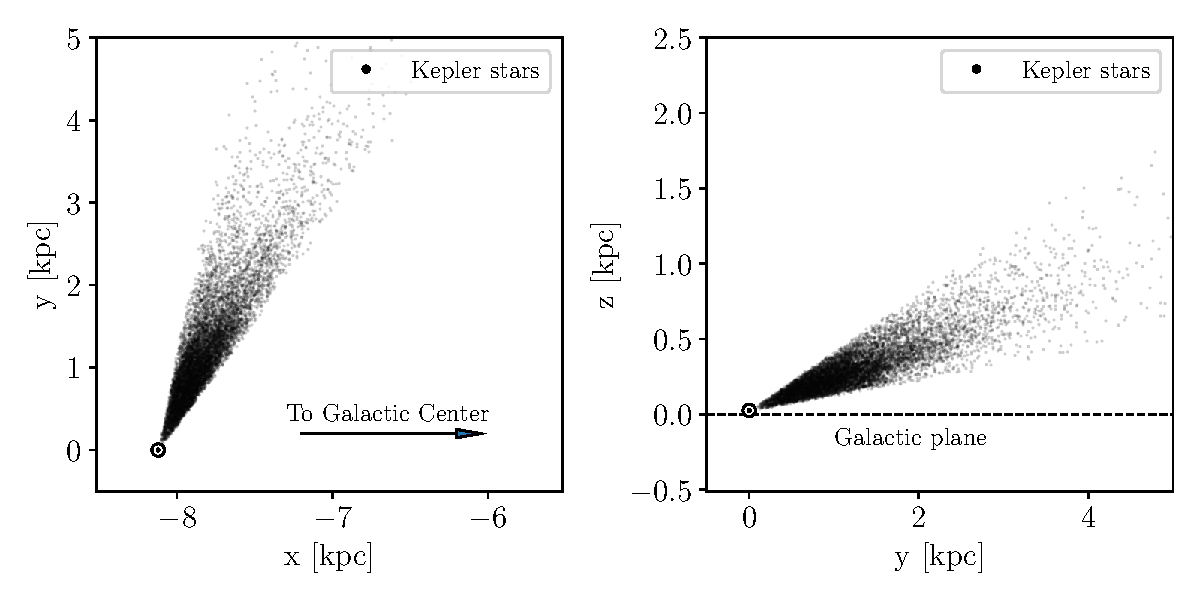
\includegraphics[width=.7\textwidth]{kepler_field}
\label{fig:kepler_field}
\end{figure}

\subsection{The prior}
\label{sec:prior}

The prior distribution over distance and velocities was constructed from the
data.
We calculated the means and covariances of the \vx, \vy, \vz\ and $\ln(D)$
distributions of stars {\it with measured RVs} and then used these means and
covariances to construct a multivariate Gaussian prior over the parameters for
stars {\it without} RVs.
Velocity outliers greater than 3-$\sigma$ were removed before calculating the
means and covariances of the distributions.
The 2-dimensional ln-distance and velocity distributions are displayed in
figure \ref{fig:prior_distributions_2D}, with 2-$\sigma$ contours shown in
blue.
\begin{figure}[ht!]
\caption{
The 2D velocity and distance distributions for stars with RV measurements,
    used to construct a multivariate Gaussian prior over velocity and
    distance parameters for stars {\it without} RVs.
2-$\sigma$ contours are shown in blue.
}
  \centering
    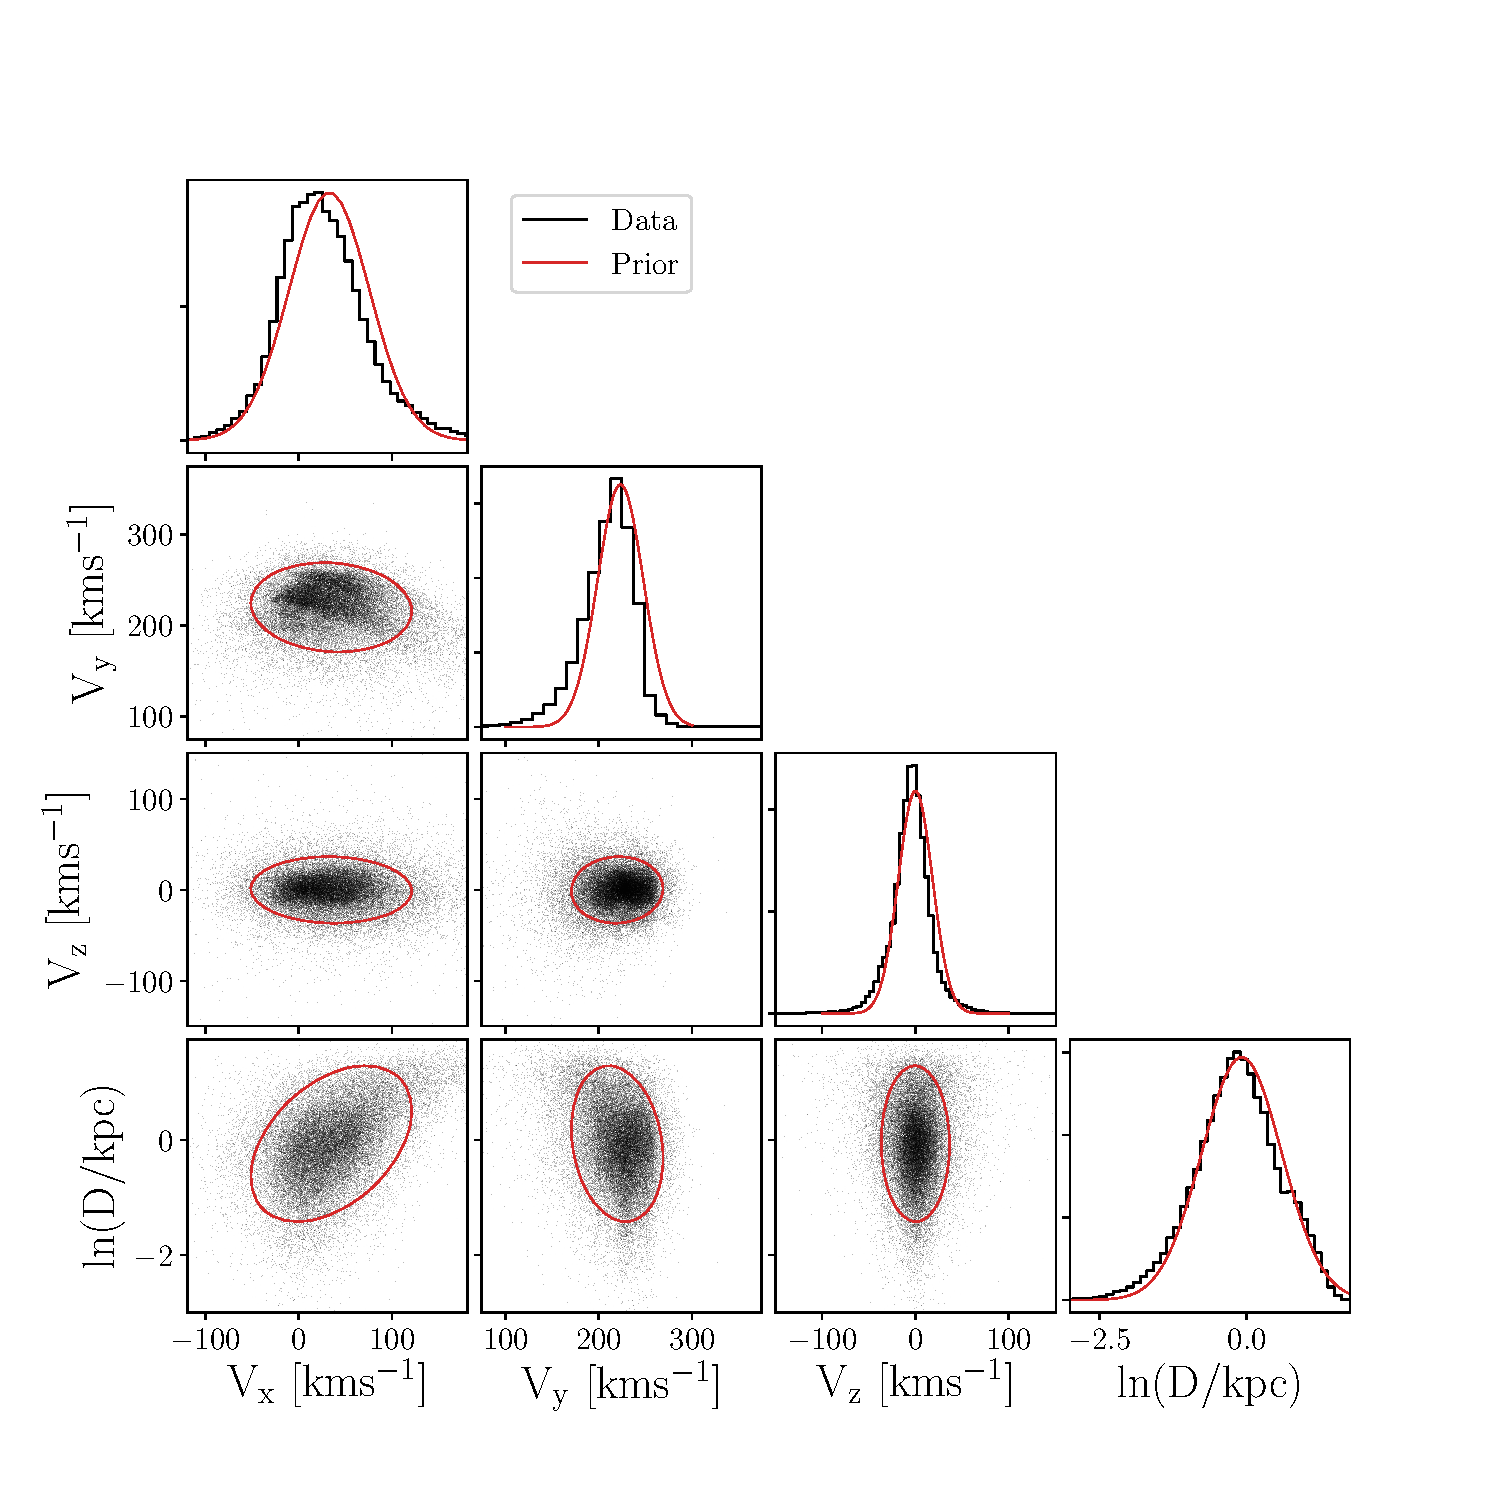
\includegraphics[width=1\textwidth]{prior_distributions_2D}
\label{fig:prior_distributions_2D}
\end{figure}

Our goal was to infer the velocities of stars {\it without} RV measurements
using a prior calculated from stars {\it with} RV measurements.
However, stars with and without RVs are likely to be different populations,
with parameters that depend on the \gaia\ and \lamost\ selection functions.
In particular, stars without RV measurements are more likely to be fainter,
cooler, and further away.
% Lower-mass stars are, on average, older, and have larger velocity dispersions,
% plus stars in different locations in the Galaxy have different orbital
% velocities.
For this reason, a prior based on the velocity distributions of stars with RVs
will not necessarily reflect the velocities of those without.
However, given that \vx\ and \vz\ are strongly informed by proper motion
measurements, and therefore likely to be relatively prior-insensitive, the
prior may not impact our final vertical velocity, and subsequent kinematic
ages, significantly.
Remember, we are mainly interested in the \vz\ parameter because {\it
vertical} velocity dispersion is a well-studied age indicator.

We tested the influence of the prior on the velocities we inferred.
One of the main features of the \gaia\ and \lamost\ RV selection functions is
brightness: \gaia\ DR2 RVs are only available for stars brighter than around
13th magnitude, and \lamost\ RVs for stars brighter than around 17th
magnitude.
\racomment{Ruth, check the actual LAMOST selection function.}
For this reason, we tested priors based on stellar populations with different
apparent magnitudes.
Three priors were tested: one calculated from the velocity distributions of
the brightest half of the RV sample (\gaia\ $G$-band apparent magnitude $<$
13.9), one from the faintest half ($G$ $>$ 13.9), and one from all stars with
RVs.
Figure \ref{fig:prior_distributions} shows the distributions of the faint
(blue) and bright (orange) halves of the RV sample as kernel density estimates
(KDEs).
The distributions are different because bright stars are more massive,
younger, and closer to the Sun on average than faint stars.
As a result, these stars occupy slightly different Galactic orbits.
The Gaussian fits to these distributions, which were used as prior PDFs, are
shown in figure \ref{prior_distributions} as dashed, colored lines.
The Gaussian fit to {\it all} the data, both bright and faint, is shown as a
black solid line.
The means of the faint and bright distributions differed by 6 \kms, 5 \kms, 1
\kms\ and 0.21 kpc, for \vx\, \vy, \vz\ and $\ln(D)$, respectively.
The \vx, \vy, and distance distributions of these stars are strongly dependent
on brightness.
However, the \vz\ distribution does not vary significantly with stellar
brightness.
Since \vz\ is the only velocity we actually used to infer kinematic ages, this
indicates that the choice of prior does not strongly impact our final results.
To confirm this, we tested the influence of the prior on the parameters.
% The black Gaussian, fit to the entire RV sample, is the prior we ended up
% using in our model.

\begin{figure}[ht!]
\caption{
    Velocity and distance distributions of faint (blue) and bright (orange)
    stars with RVs, shown as KDEs.
    Gaussian fits to these distributions are shown as dashed lines in
    corresponding colors.
    The solid black line shows the Gaussian fit to all data (bright and faint
    combined) and is the prior we ended up using in our model.
}
  \centering
    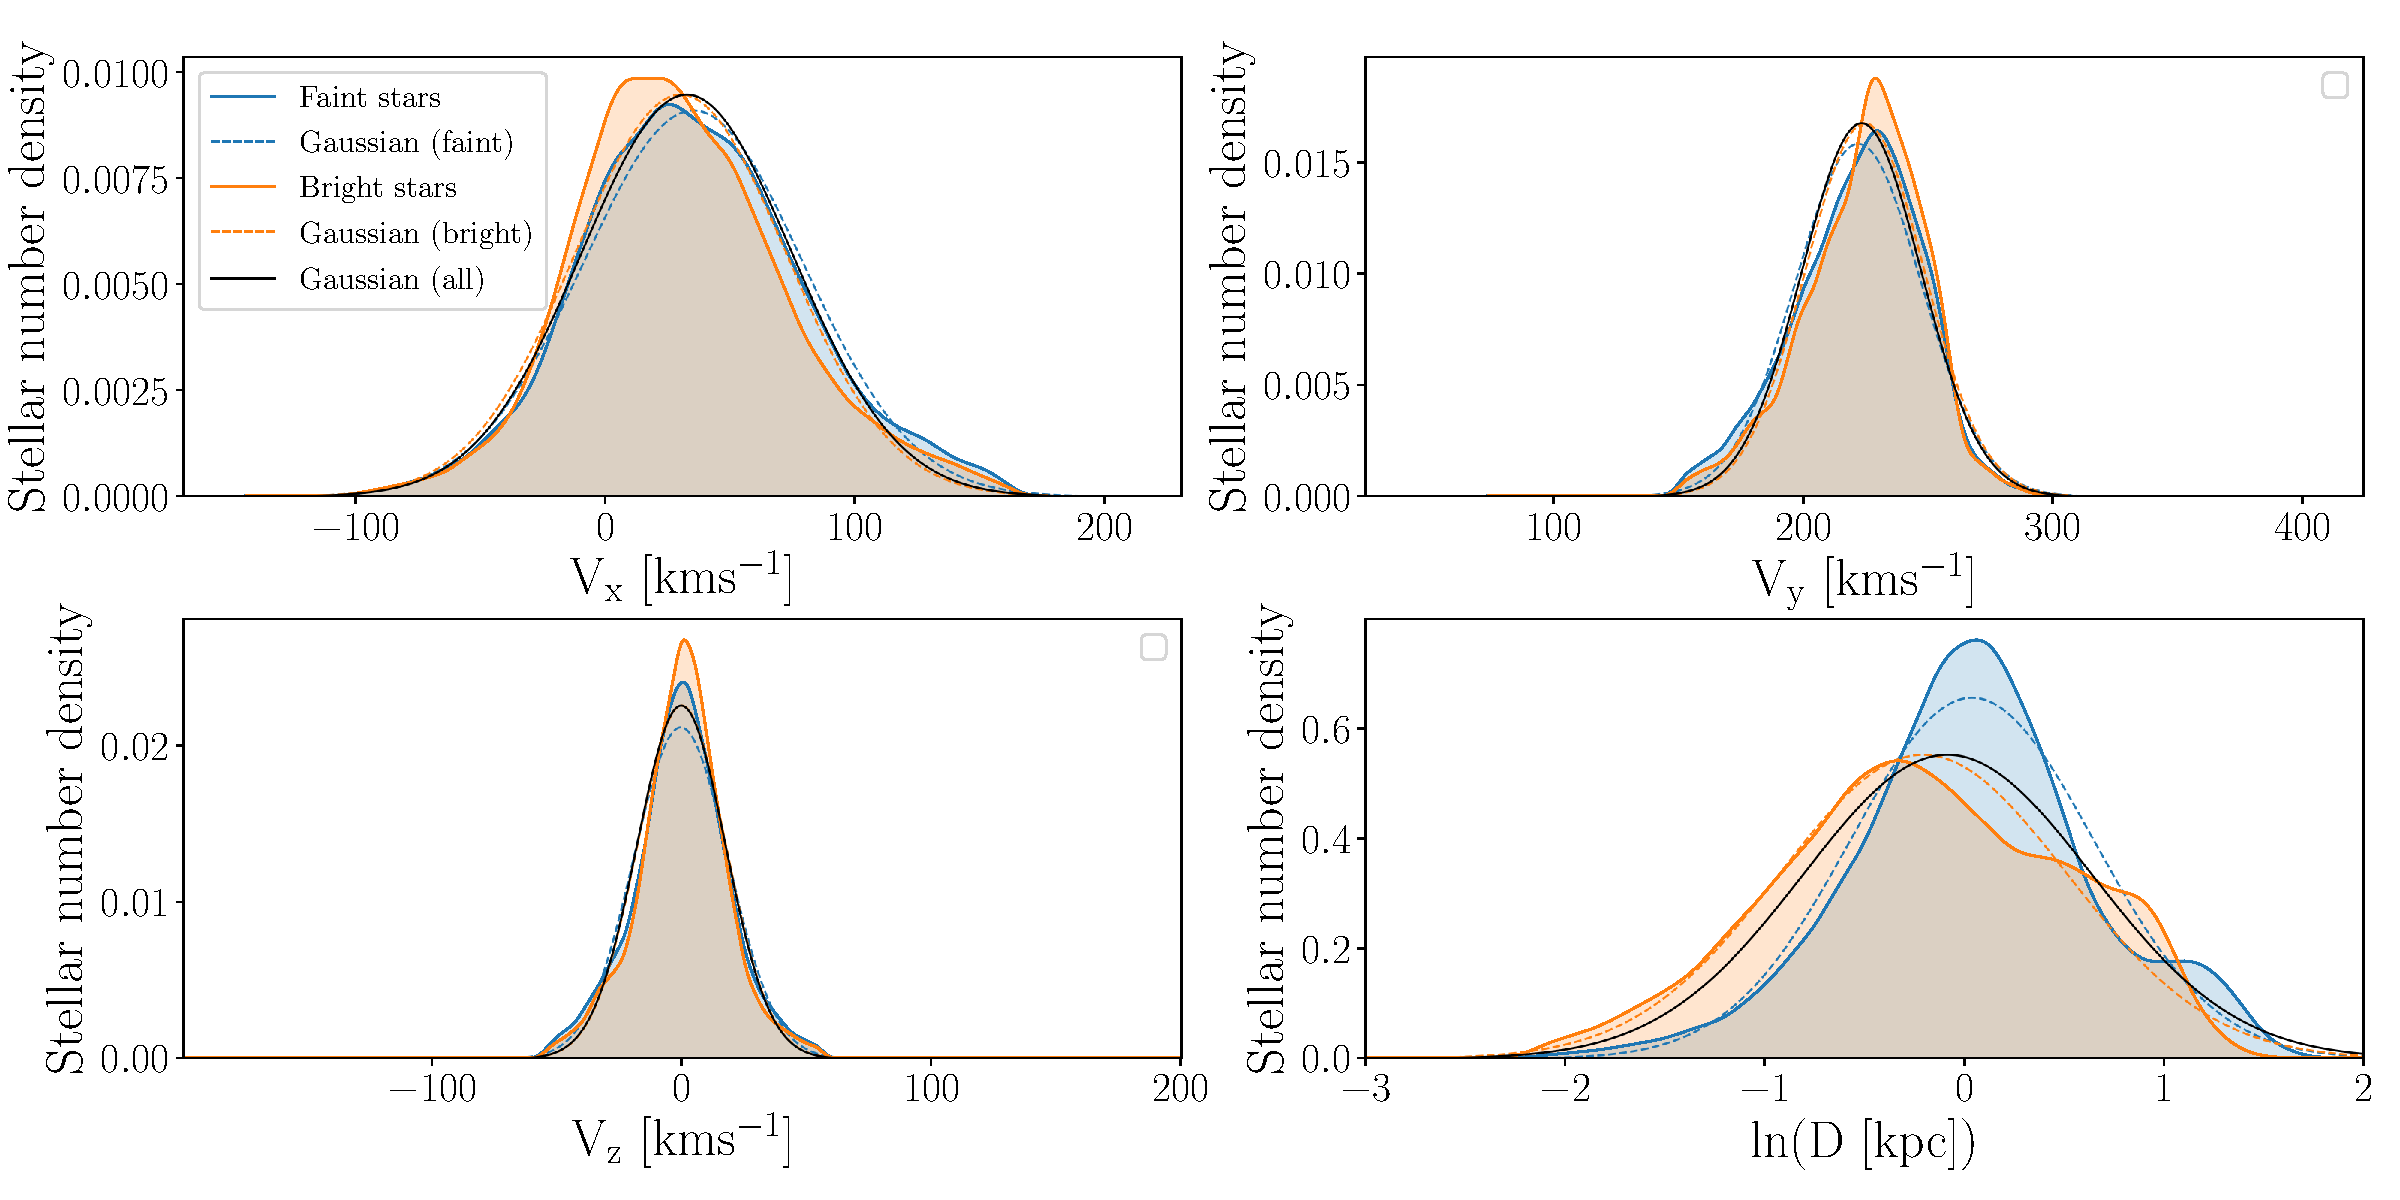
\includegraphics[width=1\textwidth]{prior_distributions}
\label{fig:prior_distributions}
\end{figure}
We inferred the velocities of 3000 stars chosen at random from the
\gaia-\lamost\ RV sample using each of these three priors and compared the
inferred velocity distributions.
If the inferred velocities were highly prior-dependent, the resulting
distributions, obtained from different priors, would look very different.
The results of this test are shown in figure \ref{fig:prior_comparison}.
From left to right, the three panels show the distributions of inferred \vx,
\vy, and \vz.
The blue dashed line shows a KDE, representing the
distributions of velocities inferred using the prior calculated from the faint
half of the RV sample.
Similarly, the solid orange line shows the distribution of inferred velocities
using the prior calculated from the bright half of the RV sample, and the
solid black line shows the results of the prior calculated from {\it all}
stars with measured RVs.

The median values of the \vy\ distributions, resulting from the faint and
bright priors, differ by around 4 \kms.
This is similar to the difference in means of the faint and bright populations
(5 \kms, as quoted above).
The inferred \vx\ and \vz\ distributions differ by 2 \kms\ and 0.3 \kms,
respectively.
Regardless of the prior choice, the \vx\ and \vz\ distributions are similar
because velocities in the \x\ and \z-directions are not strongly prior
dependent: they are tightly constrained with proper motion measurements alone.
However, the distribution of inferred \vy\ velocities {\it does} depend on the
prior.
This is because the \y-direction is close to the radial direction for \kepler\
stars (see figure \ref{fig:kepler_field}), and \vy\ cannot be tightly
constrained without an RV measurement.
% It is therefore highly dependent on the prior.
\begin{figure}[ht!]
\caption{
The distributions of velocity and distance parameters, inferred using three
    different priors.
The orange line is a KDE that represents the distribution of parameters
    inferred with a Gaussian prior, estimated from the bright half of the RV
    sample ($G < $ 13.9).
The blue dashed line shows the results from a prior estimated from the faint
    half of the RV sample ($G > 13.9$.
The black line shows the results from a prior calculated from all stars with
    RV measurements and is the prior we adopt in our final analysis.
    }
  \centering
    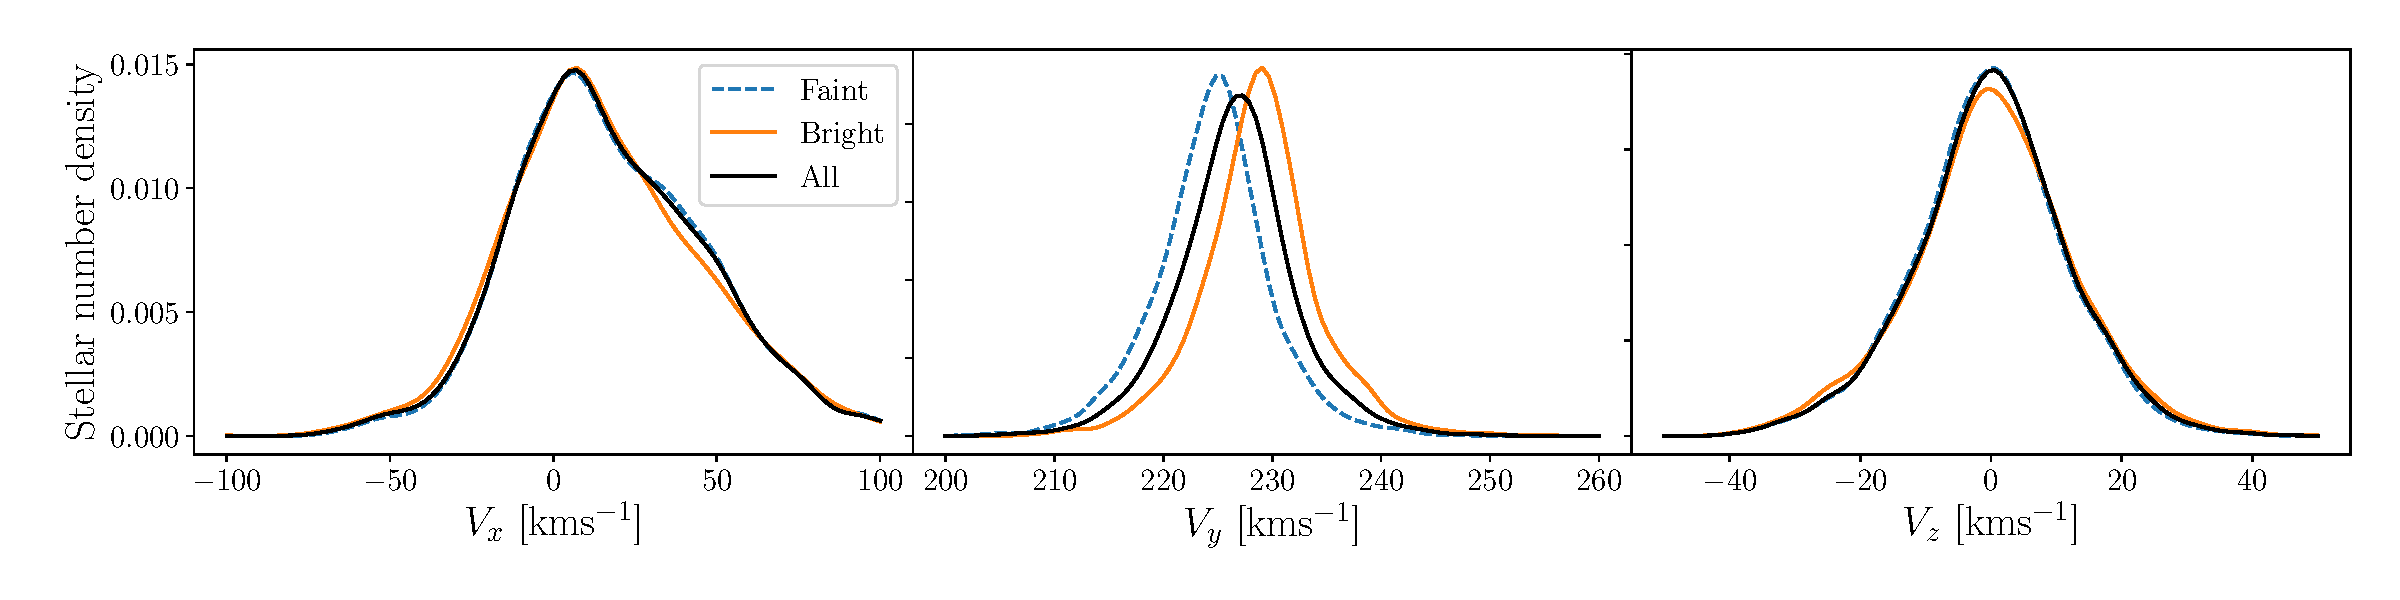
\includegraphics[width=1\textwidth]{prior_comparison}
\label{fig:prior_comparison}
\end{figure}

% Fainter stars have smaller y-velocities than brighter stars because they are,
% on average, further from the Sun

Although this test was performed on stars with RV measurements, which are
brighter overall than the sample of stars without RVs (\eg\ figure
\ref{fig:rv_histogram}), figure \ref{fig:prior_comparison} nevertheless shows
that \vx\ and \vz\ are not strongly prior-dependent.
In this work we are only concerned with \vz, as we only use {\it vertical}
velocity dispersion as an age indicator.
The difference in the dispersions of \vz\ velocities, calculated with the
three different priors tested above was smaller than 0.5 \kms.
We therefore conclude that vertical velocity dispersion is relatively
insensitive to prior choice, and we adopt a prior calculated from the
distributions of all stars with RV measurements (black Gaussians in figure
\ref{fig:prior_comparison}).

% \begin{figure}[ht!]
% \caption{
%     }
%   \centering
%     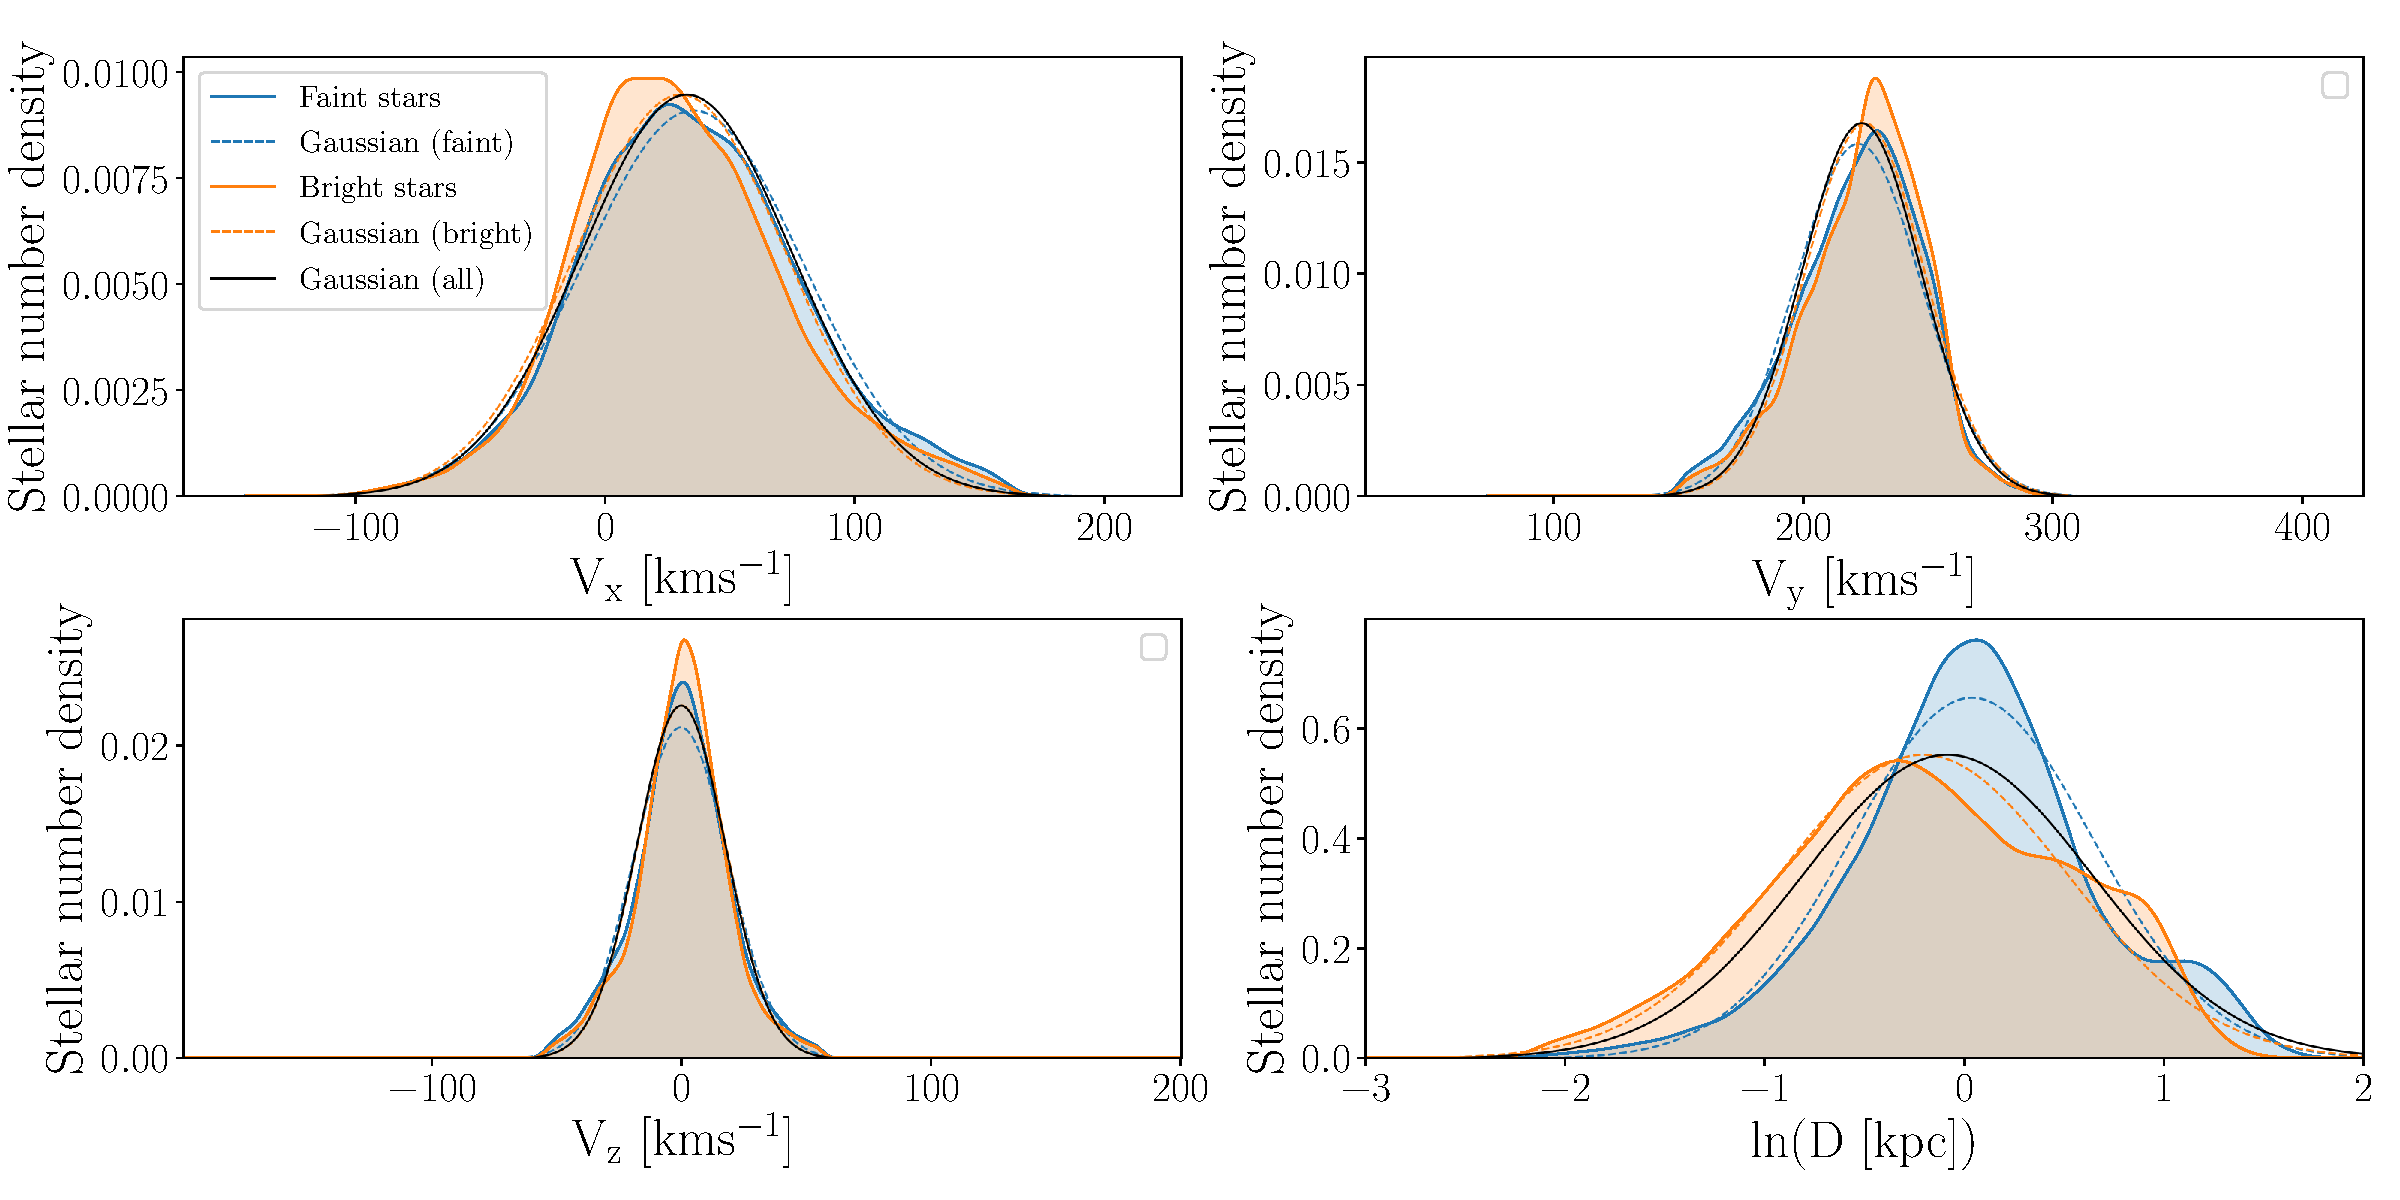
\includegraphics[width=1\textwidth]{prior_distributions}
% \label{fig:prior_distributions}
% \end{figure}

For each star in the \kepler\ field, we explored the posteriors of the four
parameters, \vx, \vy, \vz, and $\ln(D)$ using the {\it PyMC3} No U-Turn
Sampler (NUTS) algorithm, and the {\tt exoplanet} \python\ library
\racomment{(citations)}.
We tuned the {\it PyMC3} sampler for 1500 steps, with a target acceptance
fraction of 0.9, then ran four chains of 1000 steps for a total of 4000 steps.
Using PyMC3 made the inference procedure exceptionally fast -- taking just a
few seconds per star on a laptop.
\racomment{Check what convergence criteria you should use, or justify these
choices.}
